\documentclass[../root.tex]{subfiles}

\begin{document}

\section{Results}
ALTRO's performance is compared to the classic DIRCOL
method~\cite{hargraves_Direct_1987} on a number of benchmark motion-planning problems.
Each problem uses the following cost function:
\begin{align}
    J &= \frac{1}{2}(x_N - x_f)^T Q_f(x_N - x_f) \\
    &+ dt\sum_{k=0}^{N-1} \frac{1}{2}(x_k- x_f)^T Q(x_k - x_f) + \frac{1}{2}u_k^T R u_k, \notag
\end{align}
is solved to constraint satisfaction $c_{\max} = 1e\text{-}4$, and is
performed on a laptop computer with an Intel Core i7-6500U processor and 8GB
RAM. All algorithms are implemented in the Julia programming language. Unless
otherwise specified, DIRCOL is provided the dynamically feasible state
trajectory computed during the initial forward simulation from ALTRO, and
solved using Ipopt~\cite{wachter_implementation_2006}.


\subsection{Parallel Parking}
    A parallel parking problem for a Reeds-Shepp car~\cite{reeds_Optimal_1990} is
    solved with $Q = 0.001 I_{3 \times 3}$, $R = 0.01I_{2 \times 2} $, $Q_f =
    100I_{3 \times 3}$, $t_f = 3$s, and $N = 51$. Fig. \ref{ppark_runtime}
    compares the runtime performance of ALTRO and DIRCOL. ALTRO's
    unconstrained runtime is typically within a standard deviation of DIRCOL.
    ALTRO solves faster than DIRCOL for the constrained problem. Error bars
    are one standard deviation and were collected using
    \href{https://github.com/JuliaCI/BenchmarkTools.jl}{\texttt{BenchmarkTools.jl}}.
    
    A minimum-time trajectory is found by initializing both ALTRO and DIRCOL
    with the control trajectory of a solution with $t_f = 2$s and enforcing
    $-2 \leq u \leq 2$. Both algorithms converge to bang-bang control inputs
    and a minimum time of 1.54s (Fig. \ref{ppark_mintime_controls}).
    Importantly, DIRCOL failed to solve the problem several times before
    successfully finding a solution, likely due to the way Ipopt finds an
    initial feasible solution. Additionally, the DIRCOL solution rapidly
    oscillates at turning points, unlike the ALTRO solution. While DIRCOL
    converged faster in this scenario, ALTRO converged more reliably (Table
    \ref{table_performance}).
   
   \begin{figure}[t]
      \centering
      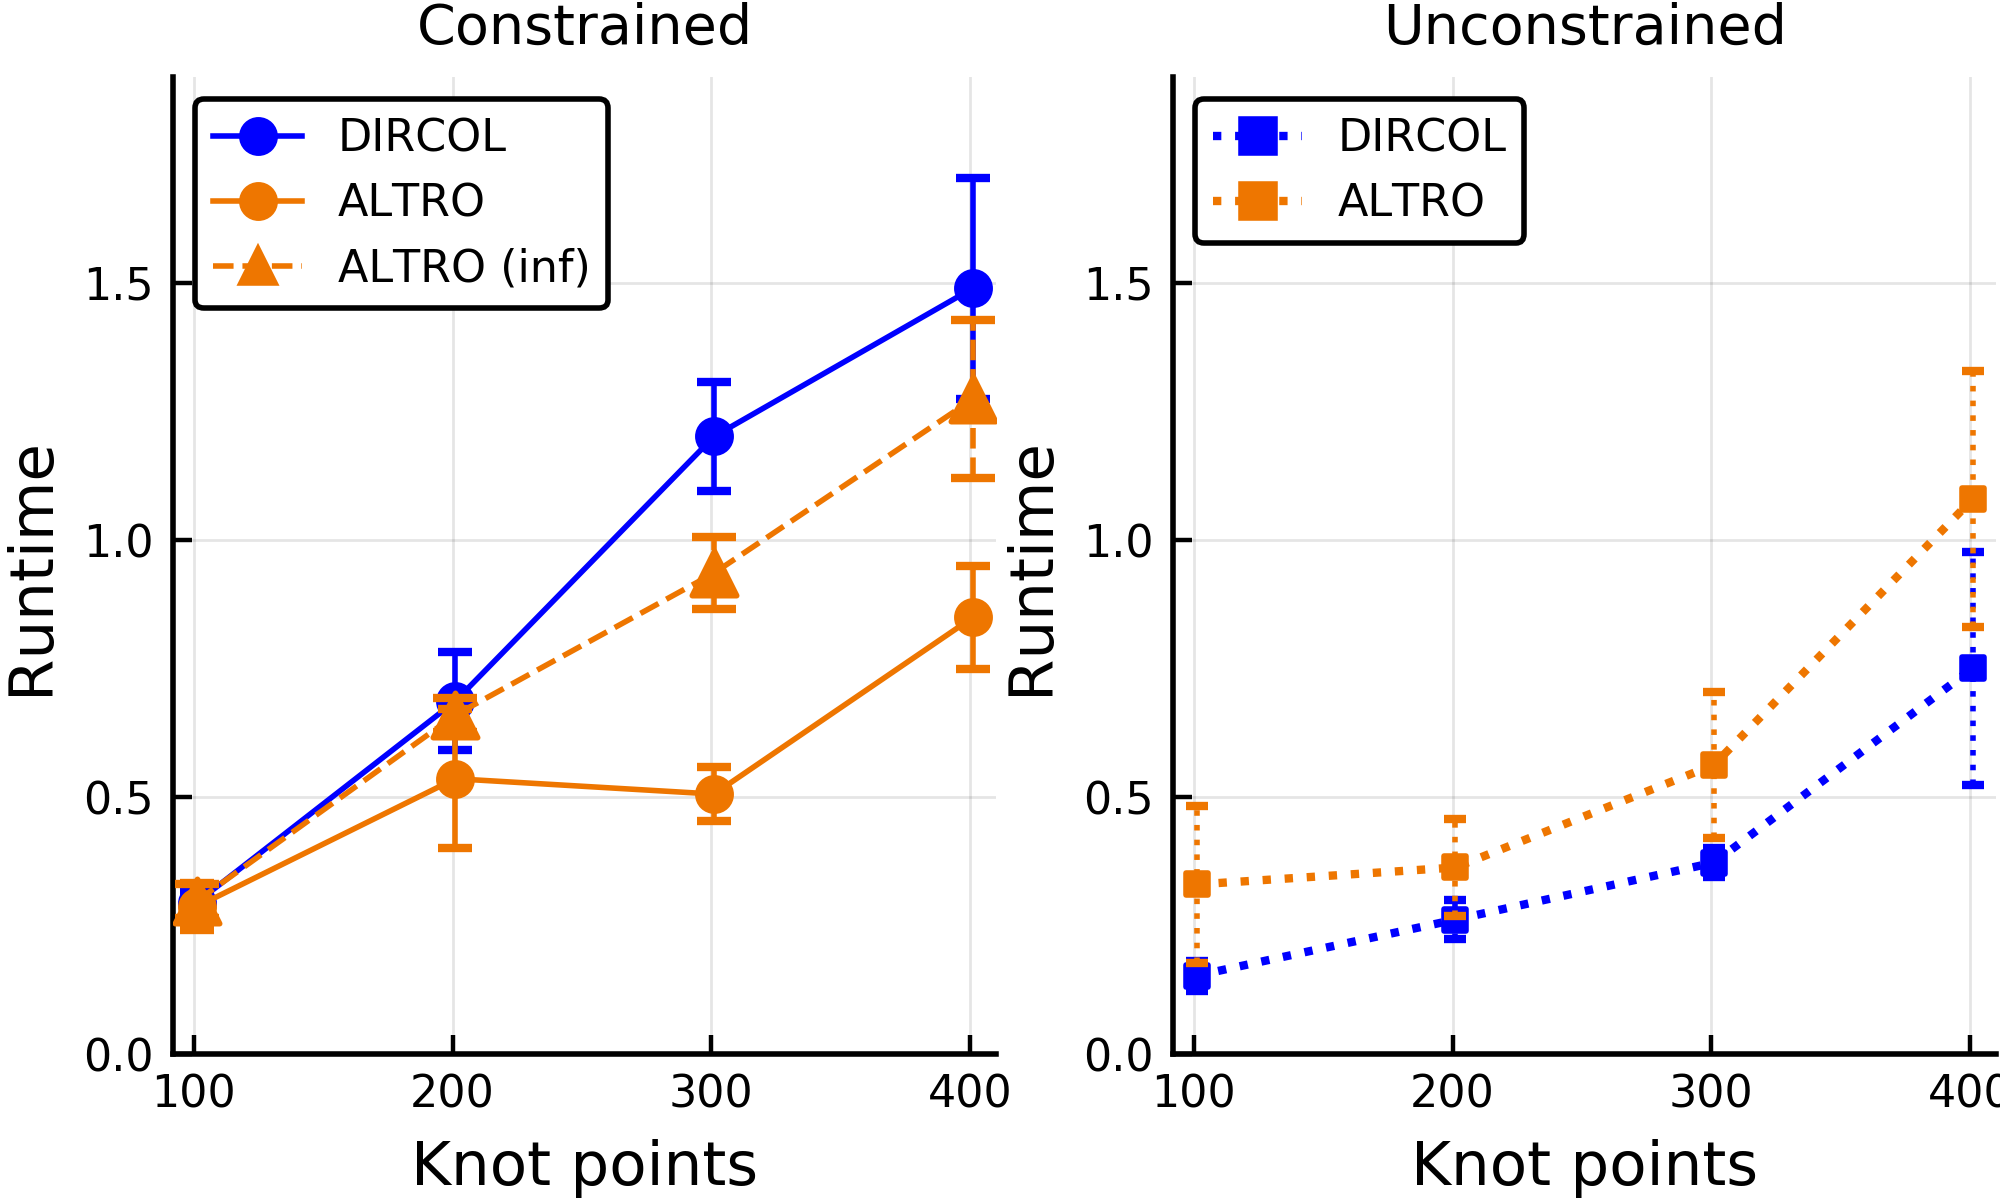
\includegraphics[width=0.75\columnwidth]{altro/ppark_runtime.png}
      \caption{Runtime comparison for parallel park problem with (left) and
      without (right) constraints.}
      \label{ppark_runtime}
   \end{figure}
   
   \begin{figure}[t]
      \centering
      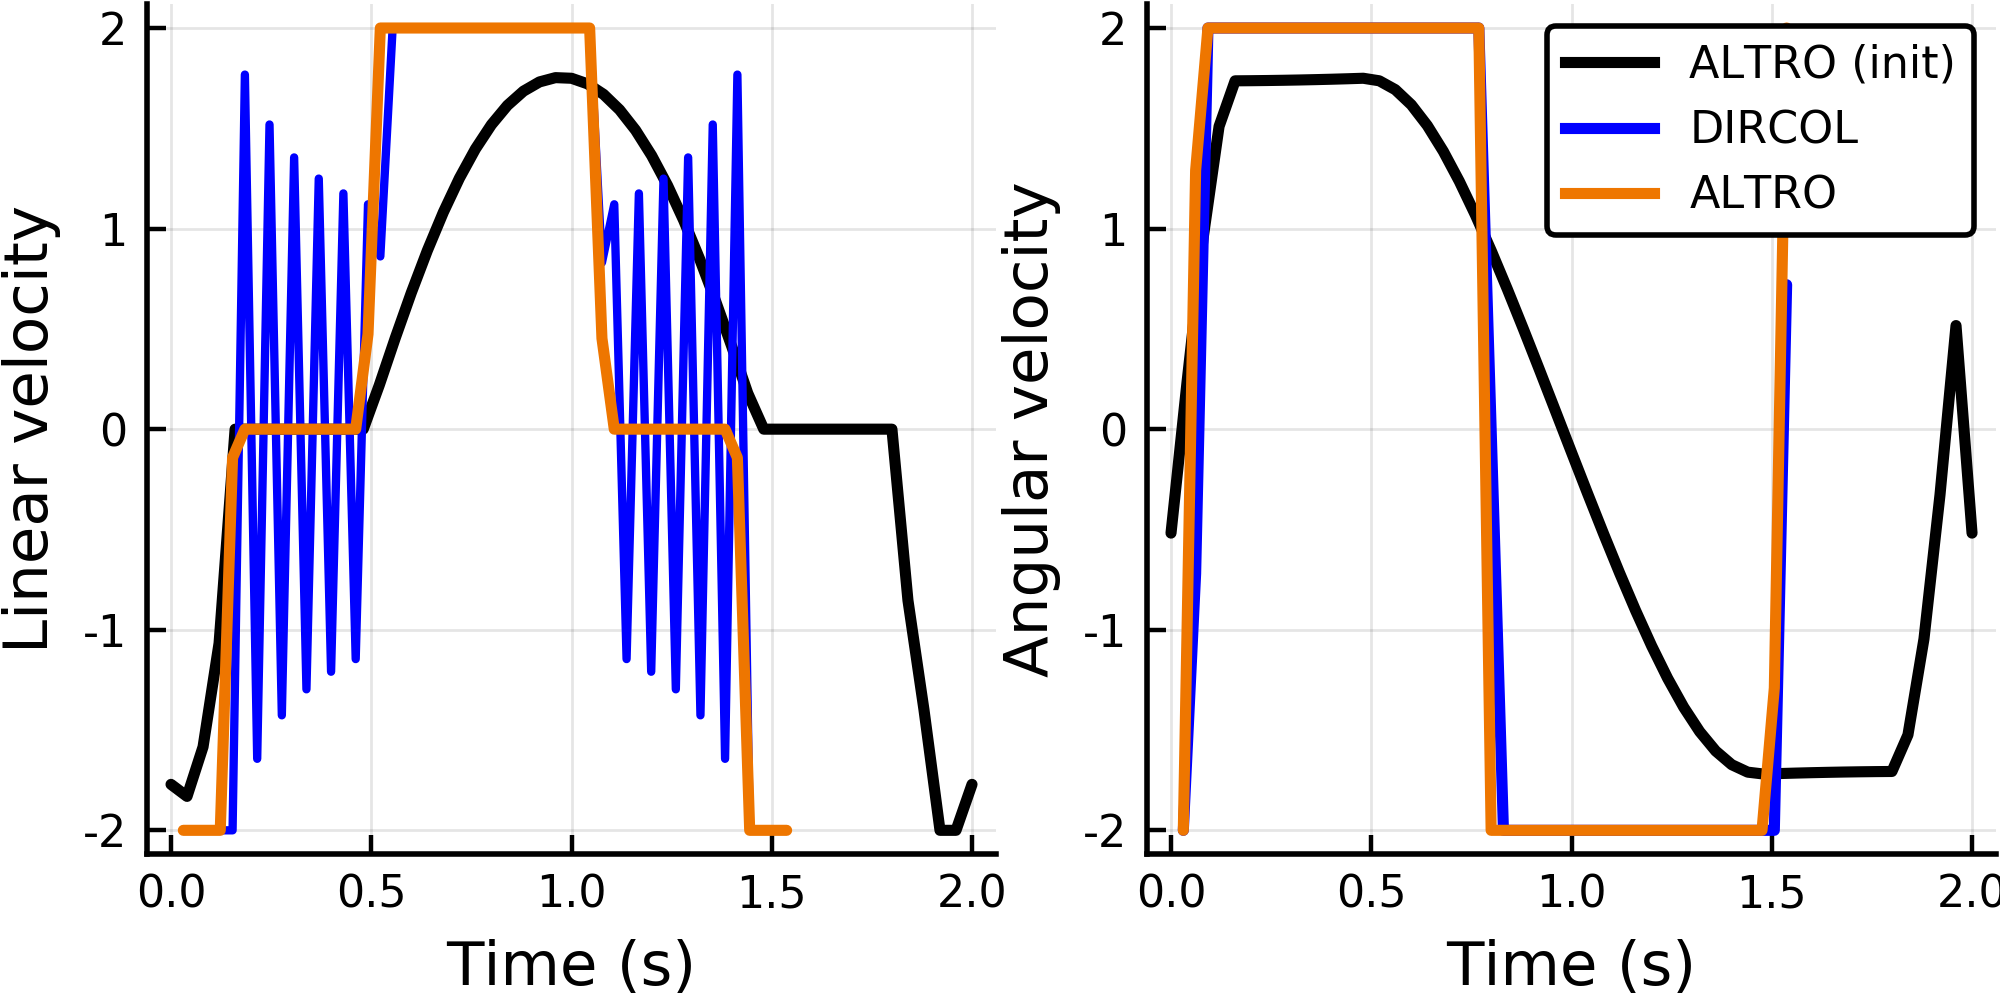
\includegraphics[width=0.75\columnwidth]{altro/ppark_mintime_control.png}
      \caption{Minimum Time Parallel Park. Fixed final time ($t_f = 2$s)
      control trajectories (black), ALTRO solution (orange), and DIRCOL
      solution (blue) for both linear and angular velocity control inputs.
      ALTRO converges to a smooth, bang-bang control, while DIRCOL exhibits
      rapid oscillation when linear velocity goes to zero (corresponding to
      the corners where the car pivots in place).}
      \label{ppark_mintime_controls}
   \end{figure}
   
%   \begin{figure}
%       \centering
%       \includegraphics[width=\columnwidth]{images/ppark_newton.eps}
%       \caption{Max constraint violation comparison for the Dubins Car parallel park scenario. Here, ALTRO$^*$ performs a single iteration of Algorithm \ref{alg:projected_newton} after $c_{\max} < 1e\text{-}6$. This iteration is relatively expensive (for our current implementation) but achieves the same constraint satisfaction as Ipopt. Without the projected Newton step, ALTRO fails to achieve constraint satisfaction below 1e-6, likely due to poor numerical conditioning.}
%       \label{ppark_newton}
%   \end{figure}

\subsection{Car Escape}
    Escape (see Fig. \ref{escape_traj}) is a problem where standard
    constrained iLQR fails to find an obstacle-free path to the goal. Using
    the same cost weights from the parallel parking problem and $N=101$, both
    ALTRO and DIRCOL are initialized with a dynamically-infeasible
    collision-free state trajectory guessed by interpolating the six points
    shown in yellow in Fig. \ref{escape_traj}. ALTRO was able to converge to
    an optimal collision-free path in less time and fewer iterations than
    DIRCOL.
    
    The projected Newton method is used to achieve high-precision constraint
    satisfaction after reaching a coarse threshold of maximum constraint
    violation $c_{\max} < 1e\text{-}3$. Fig. \ref{escape_newton} demonstrates
    ALTRO* achieving $c_{\max} < 1e\text{-}8$ in one Newton step. Runtime
    performance of this final solution-polishing step is currently relatively
    slow: The total runtime for ALTRO* is 1.398s (0.617s for the first
    stage), but should be dramatically improved with a more careful sparse
    matrix implementation. Further, Fig. \ref{escape_newton} suggests that
    this final Newton step should be initiated once the penalty reaches its
    maximum value.
    
    \begin{figure}
      \centering
      \setlength{\fboxrule}{0pt}
      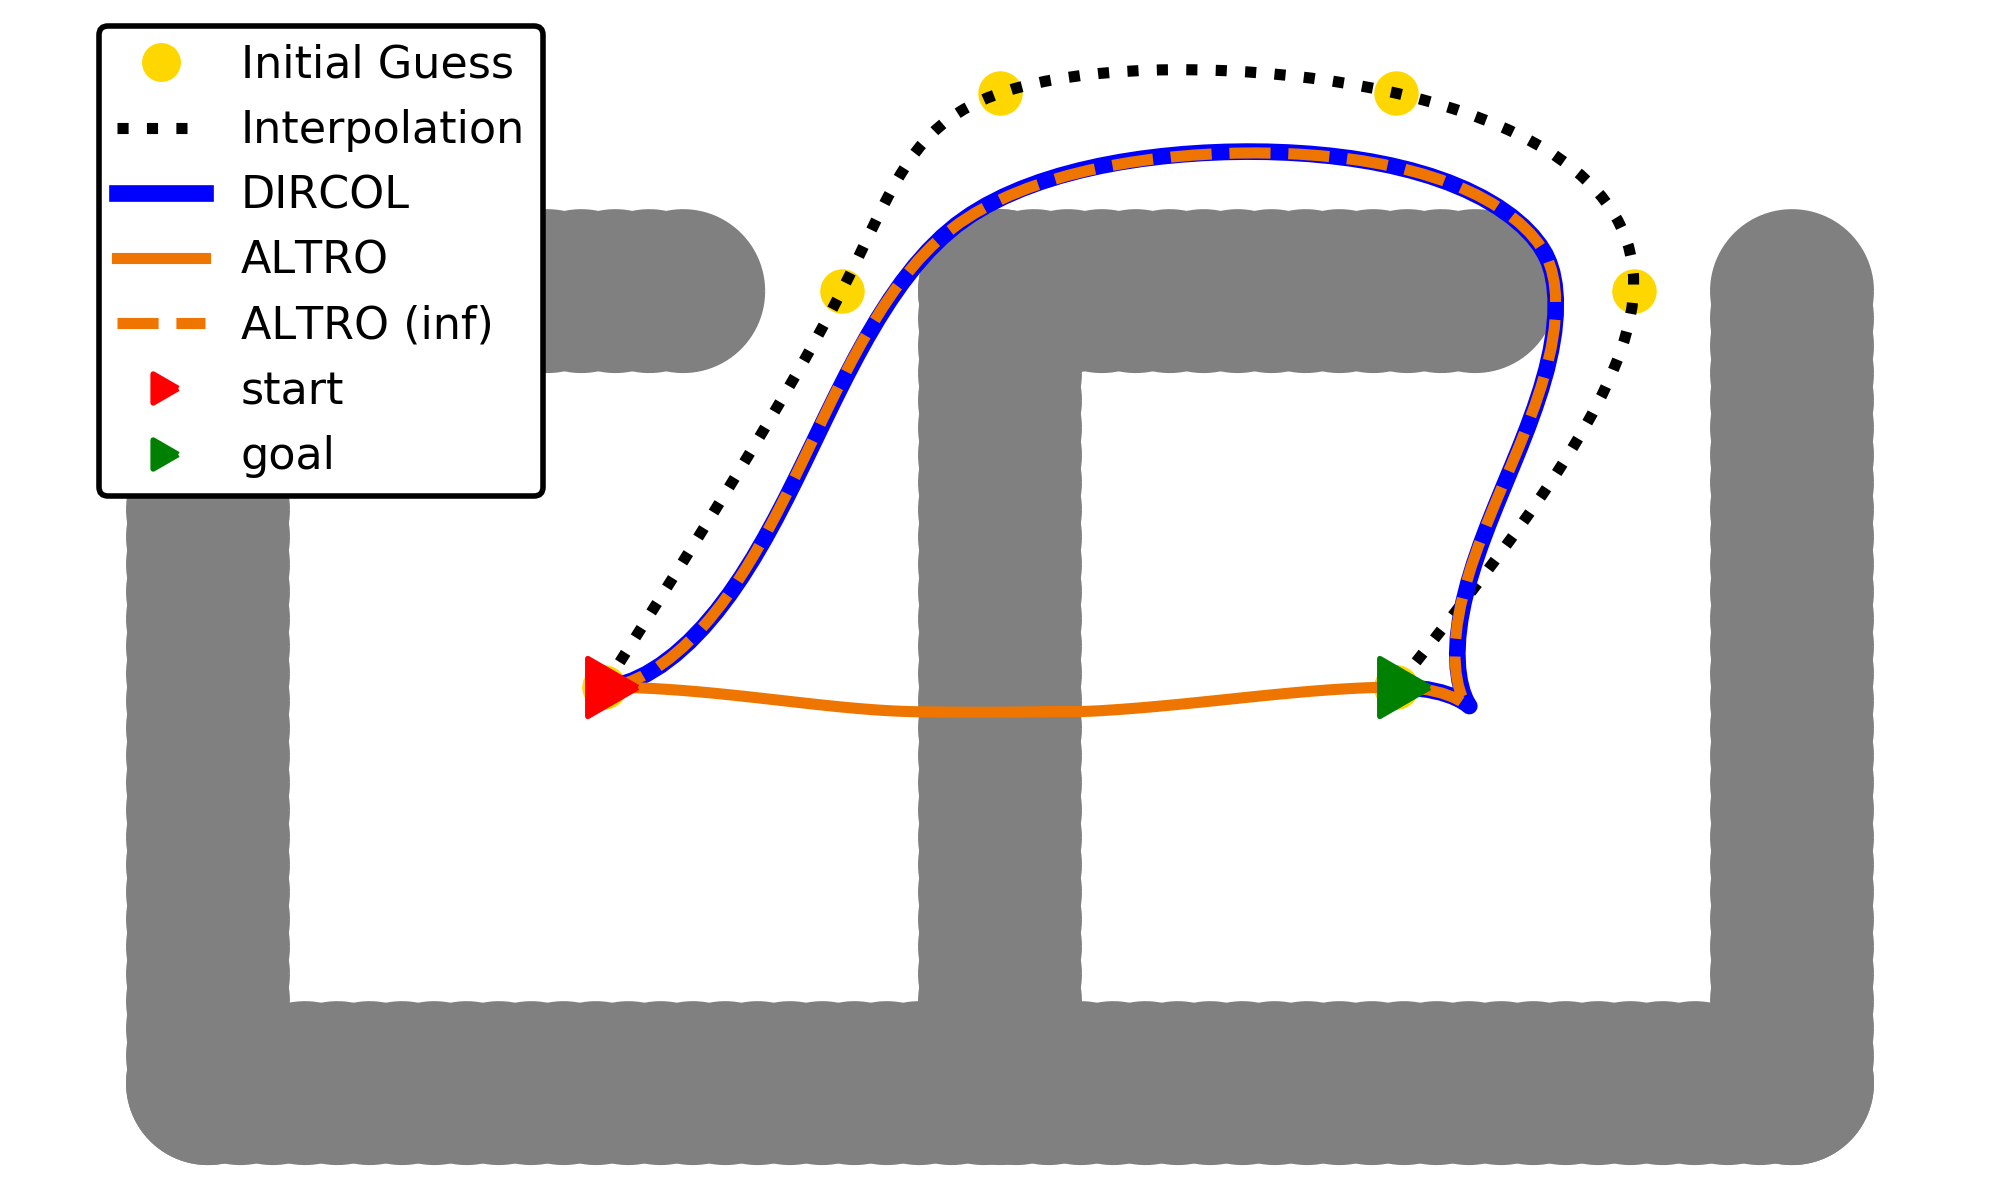
\includegraphics[width=0.75\columnwidth]{altro/escape_traj.png}
      \caption{Car Escape. The DIRCOL trajectory is blue, the (failed)
      constrained iLQR solution is solid orange, and the ALTRO solution is
      the dashed orange line.}
      \label{escape_traj}
    \end{figure}
    
    \begin{figure}
       \centering
       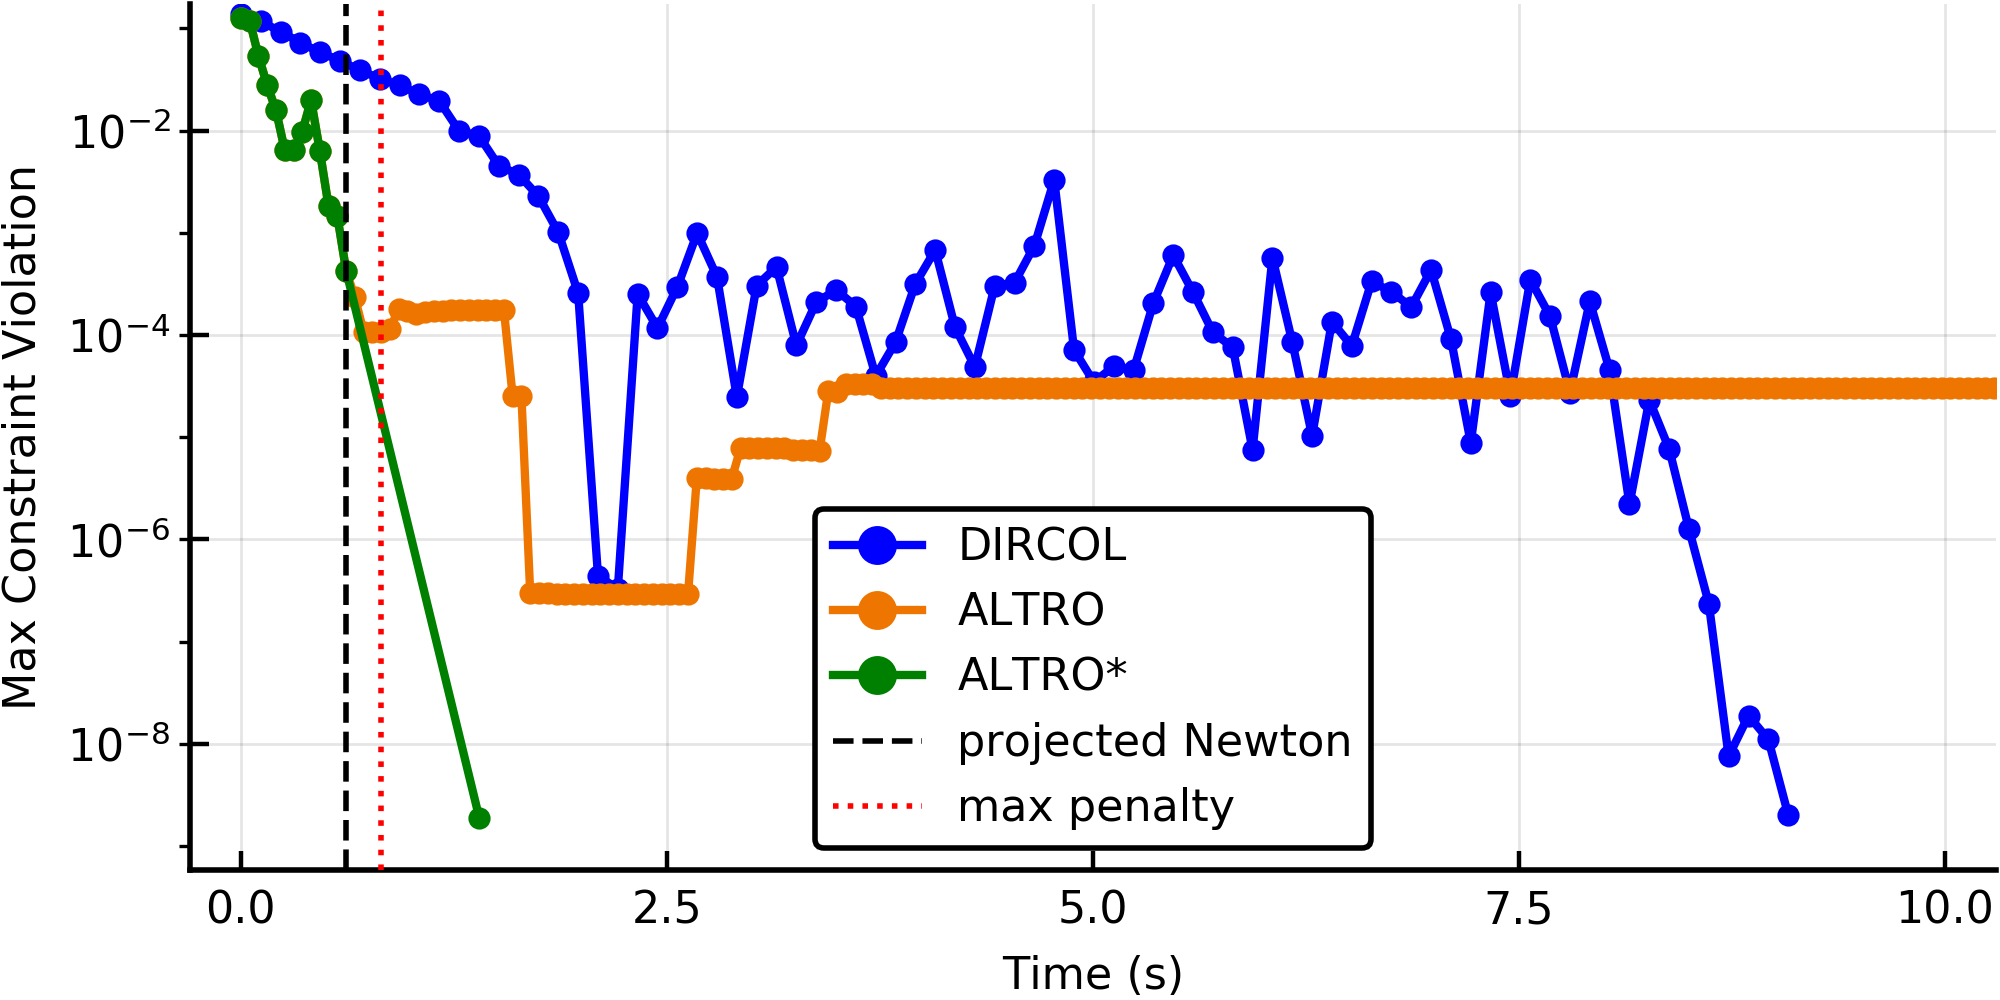
\includegraphics[width=0.75\columnwidth]{altro/escape_newton.png}
       \caption{Max constraint violation comparison for Escape. After
       reaching a coarse tolerance (dashed black line) ALTRO$^*$ performs a
       single iteration of Algorithm \ref{alg:projection}. DIRCOL
       satisfies the tolerance, but the first stage of ALTRO fails to achieve
       the desired constraint tolerance, likely due to poor numerical
       conditioning after reaching the maximum penalty (dotted red line).
       Additionally, DIRCOL finds a slightly lower cost than ALTRO$^*$, 0.331
       vs 0.333.}
       \label{escape_newton}
   \end{figure}
    
\subsection{Quadrotor Maze}
    A quadrotor is tasked with navigating the maze (with floor and ceiling
    constraints) shown in Fig. \ref{quad_infeasible}. The cost weighting
    matrices are $Q = I_{13 \times 13}$, $R = I_{4 \times 4}$, $Q_f =
    1000I_{13 \times 13}$, $t_f = 5.0$s, and $N = 101$. Input constraints, $0
    \leq u \leq 50$, are also enforced. The solvers are initialized with an
    infeasible state trajectory indicated by the yellow points in Fig.
    \ref{quad_infeasible} and inputs are initialized for hovering. ALTRO is
    able to find a collision-free trajectory, while DIRCOL fails to find
    collision-free trajectories even after being initialized with the
    solution from ALTRO (denoted by ``$+$'' in Table
    \ref{table_performance}).
    
    \begin{figure}
        \begin{subfigure}[b]{0.48\textwidth}
            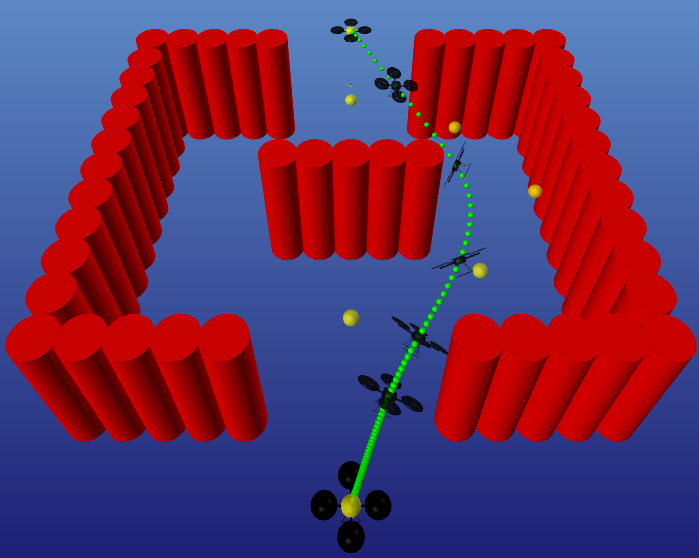
\includegraphics[width=\textwidth]{altro/quadrotor_maze_v3.png}
            \caption{}
            \label{quad_infeasible}
        \end{subfigure} 
        \hfill
        \begin{subfigure}[b]{0.48\textwidth}
            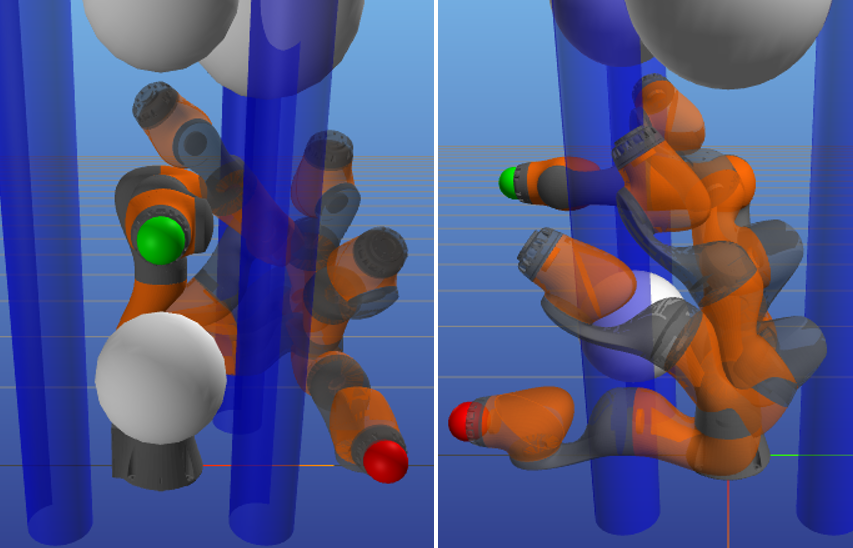
\includegraphics[width=\textwidth]{altro/kuka_combined.png}
            \caption{}
        \end{subfigure}
        \caption{3D visualizations of the quadrotor and robotic arm solutions. 
            a) Quadrotor navigating maze environment. ALTRO is
            initialized with a cubic interpolation of the yellow spheres and
            converges to the green trajectory. The quadrotor exhibits dynamic,
            aggressive banking maneuvers to avoid the obstacles.
            b) Front (left) and side (right) views of Kuka iiwa arm moving
            end effector from initial position (red) to desired position (green).
            \label{fig:kuka_snapshot}
            }
    \end{figure}
   
\subsection{Robotic Arm Obstacle Avoidance}
    A Kuka iiwa robotic arm is tasked with moving its end-effector through a
    set of closely spaced obstacles to a desired final position (see Fig.
    \ref{fig:kuka_snapshot}) using the cost function $Q = \text{diag}(I_{7
    \times 7},100I_{7 \times 7})$, $R = 0.01I_{7 \times 7}$, $Q_f = 10I_{14
    \times 14}$, $t_f = 5.0$s, and $N = 41$, subject to torque limits: $-80
    \leq u \leq 80$. The input trajectory is initialized with a stationary
    gravity-compensated trajectory. DIRCOL failed to solve this problem unless
    initialized with the ALTRO solution. Performance of ALTRO and warm-started
    DIRCOL (values denoted $^*$) are given in Table \ref{table_performance}.
   
   \begin{figure}[t]
       \centering
   \end{figure}

\begin{table}
    \caption{Peformance of ALTRO vs DIRCOL}
    \begin{center}
        \begin{tabular}{|c||c|c|c|}
            \hline
            System & Time (s) & Iters & Evals/Iter \\
            \hline
            \hline
            Parallel Park & 0.117 /\textbf{ 0.100} & 42 / \textbf{24} & \textbf{410} / 532 \\ \hline
            Parallel Park & \textbf{0.098} / 0.154 & \textbf{20} / 37 & 912 / \textbf{493} \\ \hline
            Parallel Park (m.t.) & 0.845 / \textbf{0.645} & 128 / \textbf{84} & 2176 / \textbf{465} \\ \hline
            Escape & \textbf{2.83} / 9.08  & \textbf{37} / 79 & \textbf{357} / 948 \\ \hline
            Escape (ALTRO$^*$) & \textbf{1.94} / 9.08  & \textbf{14} / 79 & \textbf{357} / 948 \\ \hline
            Quadrotor Maze & \textbf{23.0} / 559+ & \textbf{218} / 5000+ & \textbf{320} / 2630+ \\ \hline
            Robotic Arm & \textbf{14.3} / 313* & \textbf{227} / 4692* & 1050 / \textbf{822}* \\ \hline
        \end{tabular}
    \end{center}
    \label{table_performance}
\end{table}

\section{Conclusion}
We have presented a versatile high-performance trajectory optimization
algorithm, ALTRO, that combines the advantages of both direct and indirect
methods: fast convergence, infeasible state trajectory initialization,
anytime dynamic feasibility, and high-precision constraint satisfaction. Our
preliminary implementation demonstrates competitive---and often
superior---performance on a number of benchmark motion-planning problems when
compared to direct collocation implemented with the Ipopt solver. We find
that ALTRO performs particularly well in comparison to DIRCOL on problems
involving obstacles and high-dimensional state and input spaces. Future work
will focus on improving runtime performance by taking advantage of problem
sparsity and parallelization. Our implementation of ALTRO is available at
{\footnotesize
\url{https://github.com/RoboticExplorationLab/Altro.jl}}.

\end{document}